%
% File: chap02.tex
%
\let\textcircled=\pgftextcircled
\chapter{Graph Partitioning for Large Graphs}
\label{Chapter3}
This chapter is going to develop all the concepts related to the modifications made to the GAP framework. It contains the proposed solution and the principles to understand them.

\section{Node Embeddings}
As mentioned by Zhang et. al.~\cite{gcnreview}, GCN's and its variants have become a very hot topic in Machine Learning and they are being extremely used to solve plenty of problems. Indeed, the use use of Graph Convolutional Networks (GCN) to generate node embeddings was a key factor that made the GAP framework very successful in producing good quality partitions.

\subsection{Graph Convolutional Networks}
Graph Convolutional Networks were originally proposed by Kifp et. al.~\cite{gcn}. When they first came up with its algorithm, they proposed a model where a single layer follows the following propagation rule:
\begin{align}
    \label{eq:gcn}
    H^{(l+1)} = f(H^{(l)}, A) &= \sigma\left(\hat{D}^{-\frac{1}{2}}\hat{A}\hat{D}^{-\frac{1}{2}}H^{(l)}W^{(l)}\right) \\
    & H^{(0)} = X,
\end{align}
where $\boldsymbol W^{(l)}$ is a the learnable parameter weight matrix for the $l$-th network layer, $\hat{A}=A+I$ is the adjacency matrix with self loops, $\hat{D}$ is the diagonal node degree matrix of $\hat{A}$, $X$ is the feature matrix, and $\sigma$ is a non-linear activation function. Also note that the term $\hat{D}^{-\frac{1}{2}}\hat{A}\hat{D}^{-\frac{1}{2}}$ is a symmetric normalized version of the graph Laplacian.

Although GCN's are extremely powerful to generate node embeddings, in practice they have the following downsides:
\begin{itemize}
    \item In terms of efficiency, GCN's are . As it can be seen in Equation~\ref{eq:gcn}, they multiply feature matrices by powers of the graph's normalized Laplacian, i.e., they are computationally very expensive.
    \item Over-smoothing
    \item 
\end{itemize}

To solve this issues in GCN's, several solutions have been proposed that deal with the downsides mentioned without loosing expression of GCN.
FastGCN
GraphSAGE 
PinSAGE

Different approaches that can be followed are found by the author in~\cite{gnnsurvey} or~\cite{hamilton}


Describe Downsides

Mention all the approaches that use Graph Neural Networks and its importance in solving graph related tasks
achieving superior performance on many graph-related tasks


Talk a little bit about traditional node embeddings approaches and its delimitations.
 Embeddings: dense vector representations
Talk about the message passing framework
Start with Grpah Convolutional Neural Networks (GCN) and its limitations. Emphasize in how GraphSAGE solve those limitations and how it extends the GCN capabilities

\subsection{GraphSAGE}
As claimed by the authors of the paper~\cite{graphsage} where it was first proposed, GraphSAGE is an inductive framework that generate node embeddings for previously unseen data. It can be seen as an extension of the GCN framework to the inductive setting but it results advantageous in this process as it:
\begin{itemize}
    \item Performs localized convolutions without needing to use the whole normalized Laplacian resulting in a reduction of the computing time. Due to the nature of the GCN's, they make use of the symmetrically normalized graph Laplacian localized convolutions.
    \item Does not require that all nodes are present during training of the embeddings which turns out in a highly scalable framework.
    \item Naturally generalize to unseen nodes and even complete sub-graphs.
    \item Is capable of recognizing local and global structural properties of nodes based only on its neighborhood even though it still depends on node features.
    \item Uses an unsupervised loss function that tries to preserve graph structure without being specific on the task.
\end{itemize}

The basic idea of this framework to compute an embedding for node $v$ can be summarized by the following three steps:
\begin{enumerate}
    \item Sample a set of nodes from the neighborhood of $v$ uniformly at random
    \item Aggregate feature information from neighbors
\end{enumerate}

Having this idea in mind, the simplest form of a layer-wise propagation rule for GraphSAGE is given by
\begin{align}
    \label{eq:graphsage}
    \boldsymbol h_v^{(l)} &= \sigma\left(\boldsymbol W^{(l)}\cdot \textsc{Concat}\left(\boldsymbol h_v^{(l-1)},h_{N_l(v)}^{(l)}\right)\right) \nonumber \\
    \boldsymbol h_{N_l(v)}^{(l)} &= \textsc{Aggregate}_l\left(\left\{h_u^{(l-1)} \mid u\in N_l(v)\right\}\right) \\
    \boldsymbol h_v^{(0)} &= \boldsymbol  X_v \nonumber
\end{align}
where as usual $\boldsymbol W^{(l)}$ is a the learnable parameter weight matrix for the $l$-th network layer and $\sigma$ is a non-linear activation function, $\{\boldsymbol X_v \mid v\in V\}$ are the input features, $\textsc{Aggregate}_l$ are differentiable aggregator functions, and $N_l:v\rightarrow 2^V$ are neighborhood sampling functions.

After computing the node embedding for the $l$-th layer, the algorithm also performs a normalization step by dividing by the vector norm. This step is a common technique to prevent gradient explosion.

To learn the GraphSAGE parameters and get useful predictive node representations, the model can be trained in a fully unsupervised manner by using the following graph-based loss function:
\begin{equation}
    J_G(\boldsymbol z_u) = -\log\left(\sigma(\boldsymbol z_u^T\boldsymbol z_v)\right) - Q\cdot\mathbb{E}_{v_n\sim P_n(v)}\log\left(\sigma(-\boldsymbol z_u^T \boldsymbol z_{v_n})\right) 
\end{equation}

\begin{figure}[h!]
    \label{fig:graphsageloss}
    \begin{center}
        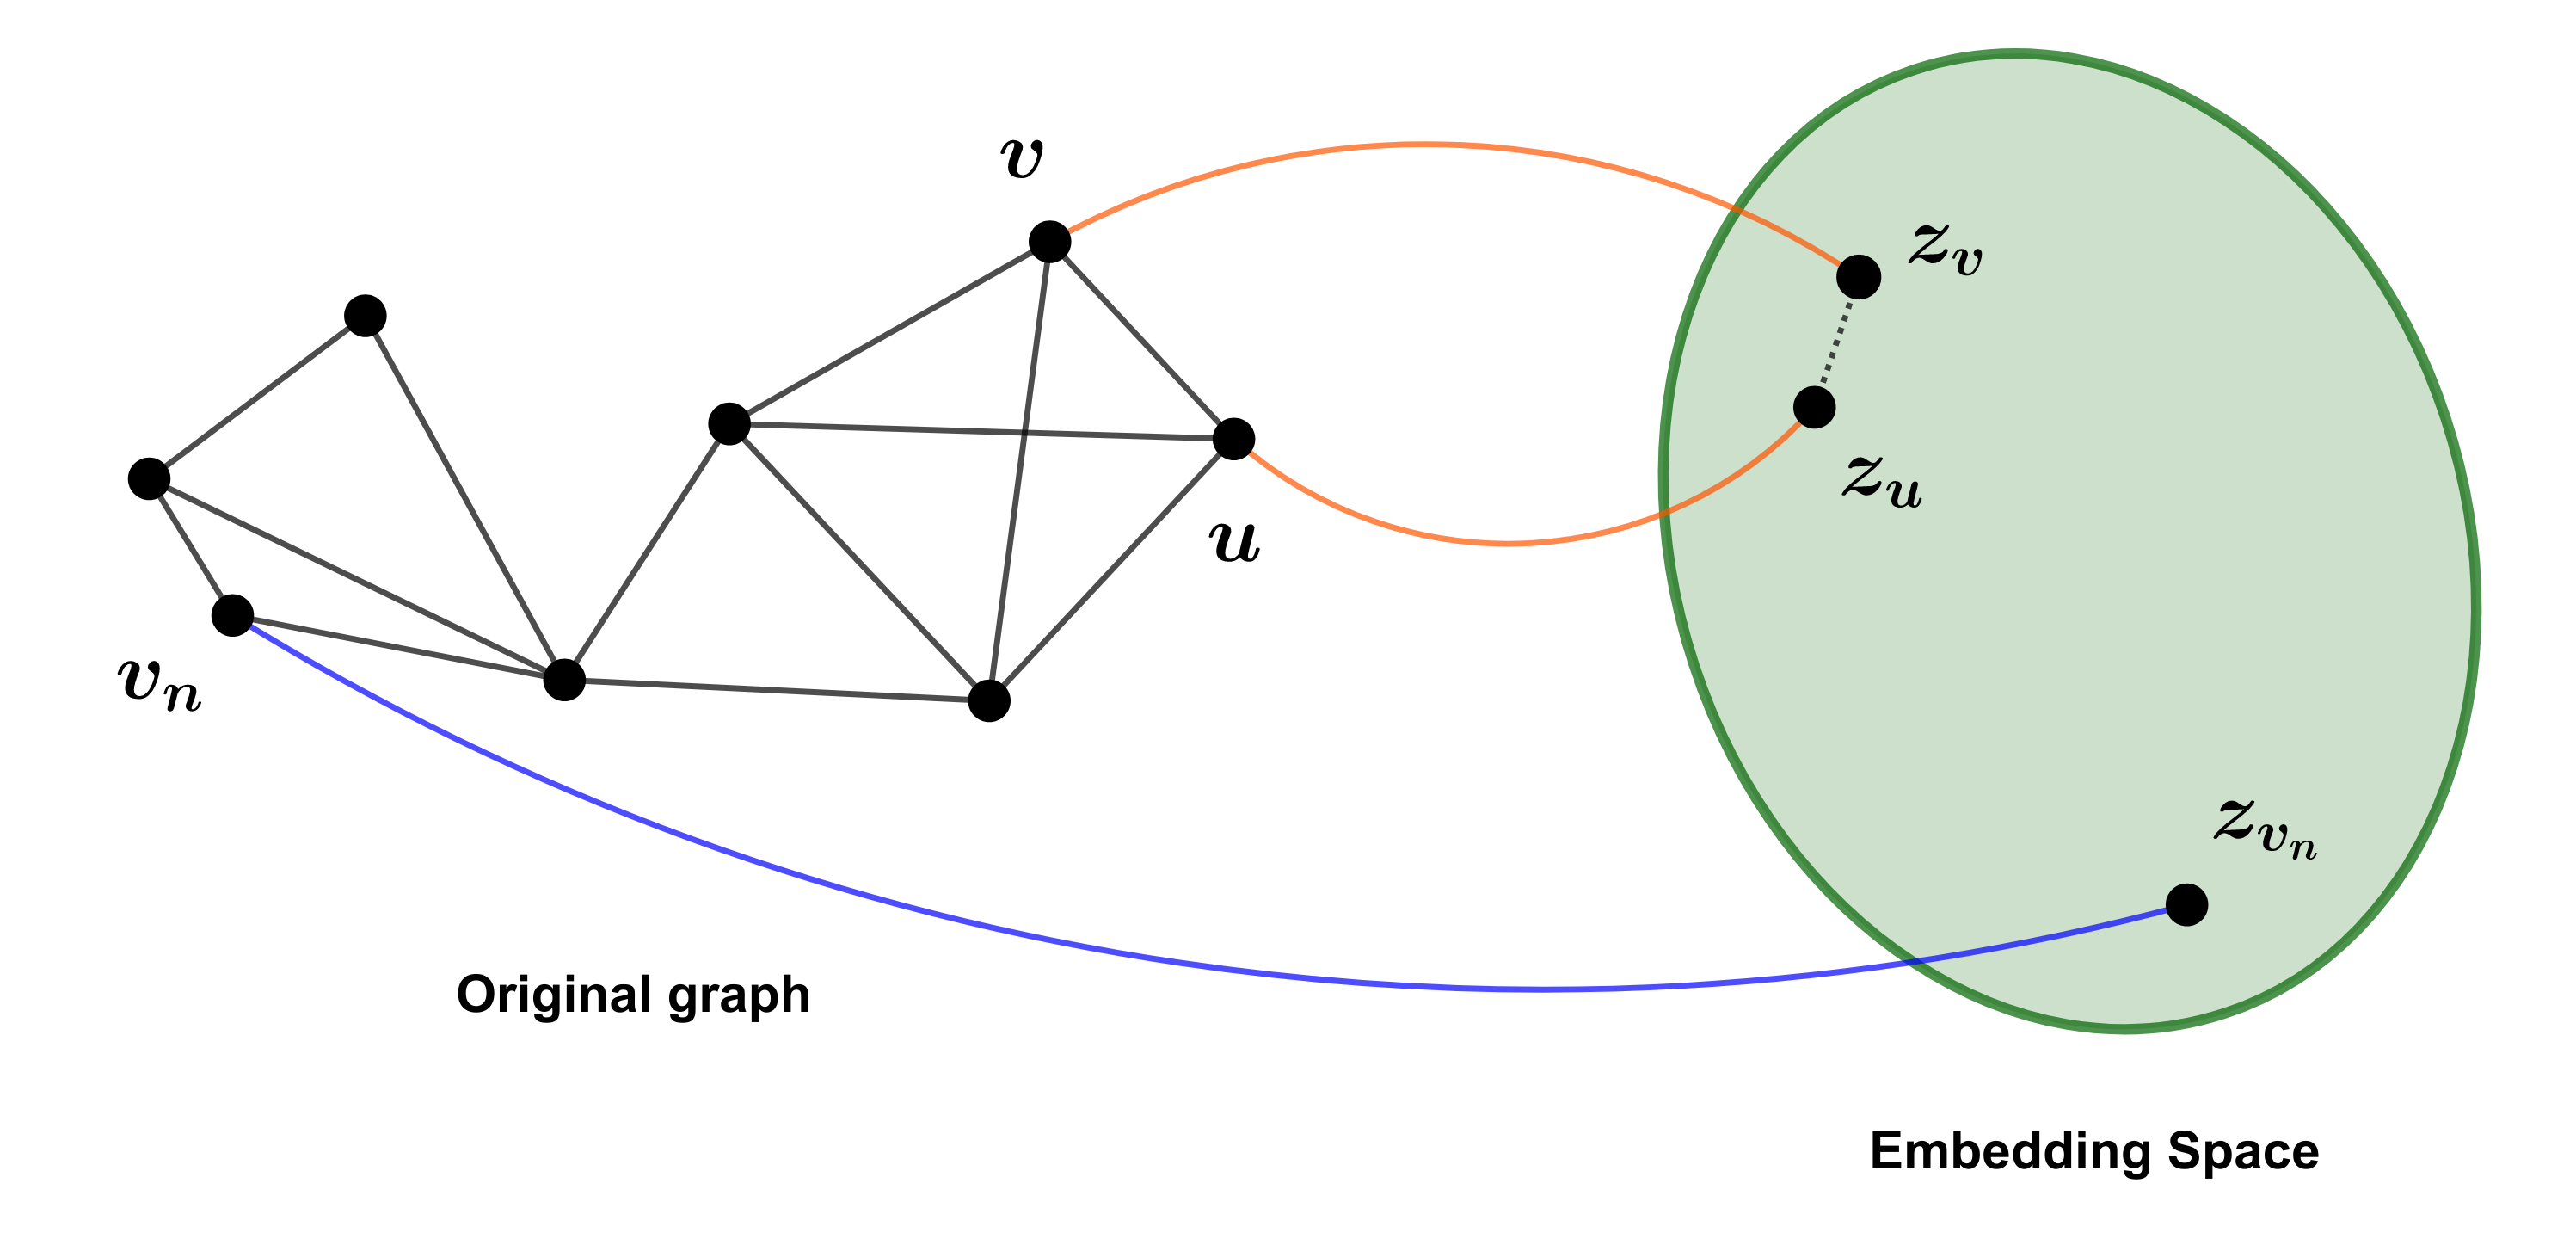
\includegraphics[scale=0.15]{graphSAGE_loss}
    \end{center}
    \caption{Graphical representation of the embeddings generated by GraphSAGE}
\end{figure}

\section{Node Features}
Many graphs come with very representative node feature information that can be very enlightening in the node embedding generation process. The key idea of Graph Neural Networks is to generate representations of nodes that depends not only on the structure of the graph but from any feature information of the graph. 

Citing textually to Chen Wang et. al.~\cite{nodefeatures}, Graph Neural Networks (GNN's) aim at learning node representations by learning the similarities shared between connected nodes. However, the expressive ability of a GNN is highly dependent on the quality of node features.

An important thing to consider is that for solving the graph partitioning problem in the version presented here, node features are irrelevant.

Due to this inherent characteristic of GNN's, and particularly of GCN's, one of the main limitations of GAP is that it requires node features.

For a graph $G = (V,E)$, where $V=\{v_1, v_2, ..., v_n\}$, the feature matrix $X$ can be described as the $n\times F$ matrix where the rows $X_{v_i}$ are that comes depending on the graph.

The way we generate node features independing task and also helps with the overall running time of the algorithm.S

GNNs aim 
Mention here: Deep Fraud Detection on Non-attributed Graph
https://arxiv.org/pdf/2110.01171.pdf
but cited here
C. T. Duong, T. D. Hoang, H. T. H. Dang, Q. V. H. Nguyen, and
K. Aberer, “On node features for graph neural networks,” arXiv preprint
arXiv:1911.08795, 2019.
[11] H. Cui, Z. Lu, P. Li, and C. Yang, “On positional and structural node
features for graph neural networks on non-attributed graphs,” arXiv
preprint arXiv:2107.01495, 2021

Eigendecomposition and top-k-eigenvalues are the k-dimensional feature vector
Q. Huang, H. He, A. Singh, S.-N. Lim, and A. R. Benson, “Combining
label propagation and simple models out-performs graph neural net-
works,” arXiv preprint arXiv:2010.13993, 2020.

Different feature initializations
http://www.cs.emory.edu/~jyang71/files/gnnfeature.pdf

\begin{center}
    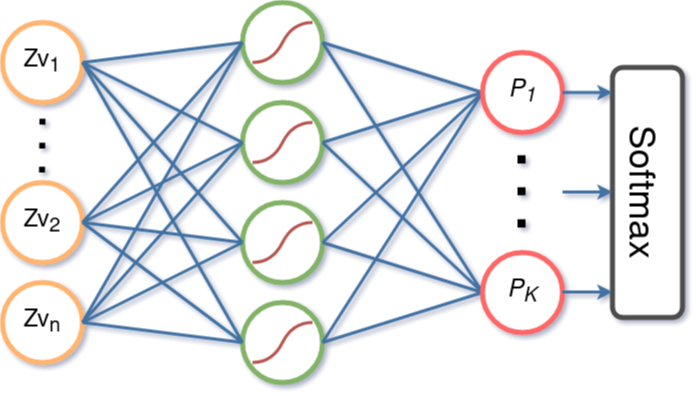
\includegraphics[scale=0.5]{partitioning_module}
\end{center}

and after playing a little bit

although GCN have been shown to extract very useful information about graph topology we need to find a different way to get that information

Some work on using Graph Neural Networks without features has been made. Use one hot representation or Initialize random feature matrices (Those methods have been shown to be equivalents and they do not generalize as mention in \cite{hamilton}. Other methods propose using applying methods as PCA to the adjacency matrix to extract the top k-eigenvalues but those approaches are computationaly very expensive, which is infeasible for large graphs and only and does not
To help capturing local information related to the graph's structure a random walk approach was chosen, have been shown efficient representation learning techniques for graphs https://arxiv.org/pdf/1901.01346.pdf, random walk kernels to produce high quality graph representations https://proceedings.neurips.cc/paper/2020/file/ba95d78a7c942571185308775a97a3a0-Paper.pdf

in particular Deep Walk to extract features about the topology of the network

According to the original paper~\cite{deepwalk}, the DeepWalk algorithm consists of two main components: a random walk generator and an update procedure. 

In the first component, a random node $v_i$ is taken uniformly at random to be the root of a random walk $\mathcal W_{v_i}$ which in its turn samples recursively from the neighbors of the last visited vertex until the maximum length $\gamma$ is reached.

As specified by Perozzi et. al.~\cite{deepwalk}, their experiments suggest that the number of walks started per vertex should be greater or equal than $\gamma=30$, the latent dimension greater or equal than $d=64$, and they fixed the sensible values of $w=10$ for the window size, and $t=40$ for the walk length . Based on those recommendations, in the experiments carried out in~\cite{deepwalk_hyper}, and the computational needs of the problem to be solved, it was found convenient to set $\gamma=60$, $d=64$, $w=15$, and $t=80$.


For the algorithm that is proposed here, the implementation by the Karate Club API~\cite{karateclub} was used.

Traditional approaches like METIS or SCOTCH implements different versions of the algorithm according to the balancedness measure, either the cardinality or the volume of the partitions. One of the great innovations presented  in~\cite{gap} is the introduction of a loss function derived from the expectation of the normalized cut. Even though they 

Ratio cut it is still used and relevant to modern research cite here https://proceedings.neurips.cc/paper/2020/file/aa108f56a10e75c1f20f27723ecac85f-Paper.pdf

or here https://www.springerprofessional.de/en/metaheuristic-approaches-for-ratio-cut-and-normalized-cut-graph-/20360832    

the authors of~\cite{gap2} proposed some modifications to GAP so it can be used for graphs without features. However the presented 

for future - Study the weighted problem
Study better features related to the problem
other ways to extract useful features for non-attributed graphs

METIS was used from the networkx interface

a table for commonly used notation

\subsection{PinSAGE and Markov Chain Negative Sampling (MCNS)}